\chapter{Présentation 1}  


{\footnotesize
\begin{itemize}
\item Logiciel\footnote{Le logiciel \emph{LibreOffice} est librement téléchargeable : \url{http://www.libreoffice.org/}. La version utilisée lors de la composition de ce document est la 5.1.} : \emph{LibreOffice Impress} 
\item Matières concernées : titulaire.
\item Compétences : 
        \begin{itemize}
        \item créer une diapositive à partir d'un modèle ; 
	\item créer une diapositive à partir d'une diapositive vide ;
	\item insérer un texte ;
	\item insérer une image ;
	\item insérer une image d'arrière-plan ;
	\item utiliser la trieuse de diapositive ;
	\item utiliser les notes de présentation ;
	\item imprimer les diapositives ;
	\item exporter les diapositives au format \texttt{PDF}.
        \end{itemize}
\item Cette fiche est à réaliser :
        \begin{itemize}
        \item avant les vacances de Noël. 
        \end{itemize}
\end{itemize}
}% fin du footnotesize



\section{Les ingrédients d'une bonne présentation}

Une présentation orale peut s'appuyer sur un diaporama qui permet d'illustrer les propos de l'orateur et lui permet de garder un fil conducteur. Attention, le diaporama est bien une illustration du discours : l'orateur ne doit jamais lire le contenu des diapositives. D'ailleurs les diapositives ne doivent pas contenir de phrase mais seulement des mots-clés, des graphiques, des schémas, des illustrations. Le diaporama ne doit pas entrer en concurrence avec l'orateur.

\subsubsection*{Mise en forme du diaporama}

\begin{itemize}
\item Choisir une ligne graphique simple, épurée, identique sur chaque diapositive.
\item Utiliser une police de caractère simple (type Arial ou Times) et de grande taille (par ex. 32 pour les textes et 44 pour les titres). Garder la même police partout.
\item Utiliser des couleurs vives à fort contraste avec le fond (texte foncé sur fond clair). Éviter les textes clairs sur fond noir qui ne se voient pas si la salle n'est pas suffisamment sombre.
\item Numéroter chaque diapositive.
\item Utiliser un minimum d'animations : elles font perdre l'attention de l'auditoire, voire l'agacent.
\item Écrire le minimum de texte : se limiter à quelques mots-clés.
\end{itemize}

\subsubsection*{Contenu du diaporama}

\begin{itemize}
\item Première diapositive : titre, prénom, nom, date et une illustration. C'est la diapositive qui est affichée avant même le début de la présentation. L'auditoire doit savoir qui parle et ce qu'il va présenter.
\item Seconde diapositive : le plan de la présentation.
\item Avant-dernière / dernière diapositive : conclusion et, si nécessaire, remerciements.
\item Entre la diapositive de titre et celle de conclusion, enchaînement logique de diapositives suivant un plan bien défini. Il faut raconter une histoire !
\end{itemize}

\subsubsection*{Deux exemples}

Comment présenter l'institut Florimont ? Ci-dessous, à gauche, une mauvaise diapositive contenant beaucoup de texte. À droite, une diapositive visuellement agréable qui ne contient que les chiffres clés et quelques icônes pour que l'orateur se souvienne de ce qu'il doit dire.

\deuximagesici{./images/presentation/diapoBad}{\textwidth}{./images/presentation/diapoGood}{\textwidth} 



\section{Les outils dont vous aurez besoin}\label{Presentation6eOutils}

Les nouveaux outils dont vous aurez besoin pour réaliser les trois séances sur la création d'une présentation sont décrits ci-dessous :


\begin{itemize}   
\item créer une nouvelle présentation, voir section \vref{Presentation1new} ;
\item créer une diapositive à partir d'un modèle, voir section \vref{Presentation1diapoModele} ;
\item utiliser la trieuse de diapositives (ordonner, dupliquer et supprimer les diapositives), voir section \vref{Presentation1trieuse} ;
\item ajouter une diapositive, voir section \vref{Presentation1nouvelleDiap} ;
\item créer une diapositive à partir d'une diapositive vide, voir section \vref{Presentation1DiapoSansModele} ;
\item insérer un texte dans une diapositive, voir section \vref{Presentation1texte} ;
\item insérer une image dans une diapositive, voir section \vref{Presentation1image} ;
\item définir une image d'arrière-plan, voir section \vref{Presentation1imageFond} ;
\item utiliser les animations, voir section \vref{Presentation1effets} ;

\item ajouter des notes de présentations, voir section \vref{Presentation1notes} ;
\item imprimer une présentation et ses notes, voir section \vref{Presentation1export} ;
\item exporter une présentation au format \texttt{PDF}, voir section \vref{Presentation1exportPDF} 
\end{itemize}  




\subsection{Créer une nouvelle présentation}\index{Impress!Créer présentation}\index{Créer présentation (Impress)}\label{Presentation1new}

Démarrer le logiciel \emph{LibreOffice} en cliquant sur la loupe en haut à droite du bureau (figure ci-dessous à gauche) puis en indiquant \texttt{LibreOffice} dans la boîte de dialogue qui s'ouvre alors. Terminer en sélectionnant \emph{LibreOffice} puis en appuyant sur la touche \texttt{Entrée} ou en cliquant à l'aide de la souris (figure ci-dessous à droite).

\deuximagesici{./images/presentation/Impress_01Ouvrir_01}{\textwidth}
              {./images/presentation/Impress_01Ouvrir_02}{\textwidth}

Une fois le logiciel ouvert, choisir dans la fenêtre d'accueil \texttt{Présentation Impress} (figure ci-dessous).

\uneimageici{./images/presentation/Impress_01Ouvrir_03}{.4\textwidth}











\subsection{Une diapositive à partir d'un modèle}\index{Impress!Diapositive à partir modèle}\index{Diapositive à partir modèle (Impress)}\label{Presentation1diapoModele}

La première chose à faire est d'afficher les modèles de diapositives. Pour cela, cliquer sur la poignée au milieu du bord droit de l'écran (figure ci-dessous à gauche), puis sélectionner l'icône des propriétés (figure ci-dessous à droite).

\deuximagesici{./images/presentation/Impress_02Creer_00}{.5\textwidth}
	      {./images/presentation/Impress_02Creer_00b}{.15\textwidth}

Dans le panneau latéral à droite de l'écran (figure ci-dessous) choisir un modèle de diapositive à trois cadres \circled{1} en double-cliquant dessus. Le modèle choisi apparaît alors dans la fenêtre principale \circled{2}. 

\uneimageici{./images/presentation/Impress_02Creer_03}{.5\textwidth}

Le modèle proposé permet l'insertion très facile de textes et d'images.

% \uneimageici{./images/presentation/Impress_02Creer_02}{.6\textwidth}

\paragraph{Insérer un texte} en cliquant sur 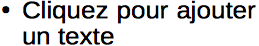
\includegraphics[width=3cm]{./images/presentation/Impress_02Creer_04}

Le texte est tapé directement dans la diapositive \circled{1} (figure ci-dessous) et les options de mise en forme (gras, italique, etc.) sont disponibles à droite de l'écran \circled{2}. 

\uneimageici{./images/presentation/Impress_03Inserer_05}{.4\textwidth}


\paragraph{Insérer une image} en cliquant sur la partie inférieure droite de l'icône 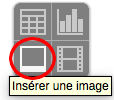
\includegraphics[width=2cm]{./images/presentation/Impress_03Inserer_01}

Dans la boîte de dialogue qui s'ouvre, rechercher le fichier qui contient l'image à insérer et terminer en appuyant sur le bouton \texttt{Ouvrir}.

\vspace{1em}

L'image peut être redimensionnée et tournée :\label{poigneeTourneZoom} 

\begin{itemize}
\item pour \textbf{redimensionner l'image}, cliquer une fois dessus et utiliser les \textbf{poignées carrées} qui apparaissent (figure ci-dessous à gauche) ;
\item pour effectuer une \textbf{rotation de l'image}, cliquer lentement deux fois dessus et utiliser les \textbf{poignées rondes} qui apparaissent (figure à droite).
\end{itemize}

\deuximagesici{./images/presentation/Impress_03Inserer_06}{.65\textwidth}
	      {./images/presentation/Impress_03Inserer_07}{.65\textwidth}




À tout moment il est possible de passer d'un modèle de diapositive à un autre modèle contenant davantage de cadres. Les figures ci-dessous montrent le passage d'une diapositive contenant un titre et trois cadres (à gauche) à une diapositive contenant un titre et quatre cadres (à droite) : l'image et le texte précédemment insérés sont conservés.

\deuximagesici{./images/presentation/Impress_03Inserer_0a}{.9\textwidth}
              {./images/presentation/Impress_03Inserer_0b}{.9\textwidth}








\subsection{Trieuse de diapositives (ordonner, dupliquer et supprimer les diapositives)}\index{Impress!Trieuse de diapositive}\index{Trieuse de diapositive (Impress)}\index{Impress!Dupliquer une diapositive}\index{Impress!Ordonner les diapositives}\index{Ordonner les diapositives (Impress)}\index{Impress!Dupliquer une diapositive}\index{Dupliquer une diapositive (Impress)}\index{Impress!Supprimer une diapositive}\index{Supprimer une diapositive (Impress)}\label{Presentation1trieuse}


\begin{minipage}[c]{.68\textwidth}
Sur la gauche de l'écran (figure ci-contre) la \emph{trieuse de diapositives} permet de naviguer rapidement d'une diapositive à l'autre, mais également de déplacer des diapositives (en manipulant les miniatures des diapositives à la souris), de dupliquer une diapositive existante (en effectuant un clic droit dessus) ou encore de supprimer une diapositive.

\vspace{1em}

Remarque : si la trieuse n'est pas visible, il faut cliquer sur la poignée pour la faire apparaître (voir \circled{1} sur la figure ci-contre).

\end{minipage}\hfill%
\begin{minipage}[c]{.3\textwidth}
\centering%
\uneimageici{./images/presentation/Impress_05Trieuse_01}{.8\textwidth}
\end{minipage}













\subsection{Ajouter une diapositive}\index{Impress!Créer diapositive}\index{Diapositive, créer (Impress)}\label{Presentation1nouvelleDiap}

Pour ajouter une diapositive, deux solutions sont possibles :

\begin{itemize}
\item un clic droit sur une diapositive dans la trieuse permet de choisir d'insérer une nouvelle diapositive ou de dupliquer la diapositive sélectionnée (figure ci-dessous à gauche) ;
\item un clic droit sur une zone vide de la trieuse permet d'insérer une nouvelle diapositive ou de coller une diapositive précédemment copier à l'aide de \texttt{Cmd + C} (figure à droite).  
\end{itemize}

\deuximagesici{./images/presentation/Impress_04NouvelleDia_02}{.65\textwidth}
	      {./images/presentation/Impress_04NouvelleDia_03}{.65\textwidth}





\subsection{Diapositive à partir d'une diapositive vide}\index{Impress!Diapositive sans modèle}\index{Diapositive à partir d'une diapositive vide (Impress)}\label{Presentation1DiapoSansModele}


\begin{minipage}[c]{.58\textwidth}
Si aucun des modèles proposés ne convient à ce que l'on souhaite réaliser, on peut partir d'une diapositive vide. Par exemple, la diapositive montrée sur la figure ci-contre est réalisée à partir d'une diapositive vide plutôt qu'à partir d'un modèle.

\subsubsection{Insérer un texte dans une diapositive}\index{Impress!Insérer un texte}\index{Texte, insérer (Impress)}\label{Presentation1texte}
\end{minipage}\hfill%
\begin{minipage}[c]{.38\textwidth}
\centering%
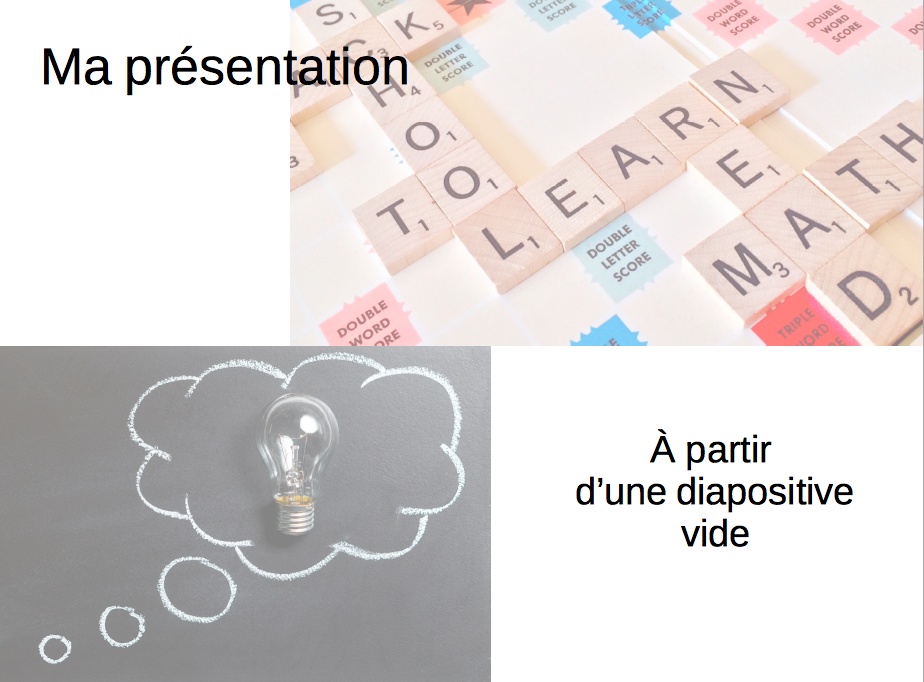
\includegraphics[angle=0,width=.75\textwidth]{./images/presentation/Impress_07DiaSansFormat_10}
\end{minipage}

\vspace{1em}


La première étape est de sélectionner une diapositive vide dans le panneau latéral à droite des modèles de diapositive (\circled{1} sur la figure ci-dessous).

On peut ensuite ajouter un texte sur la diapositive en utilisant l'outil \texttt{Zone de texte} (\circled{2} sur la figure ci-dessous).

\uneimageici{./images/presentation/Impress_07DiaSansFormat_02}{.7\textwidth}

Cliquer sur la diapositive pour écrire un texte (\emph{\og Ma présentation \fg} en \circled{1} sur la figure ci-dessous). Le panneau latéral à droite de l'écran (\circled{2}) contient toutes les options de mise en forme du texte. En cliquant sur le texte on fait apparaître des poignées qui permettent de l'agrandir ou d'effectuer une rotation, comme expliqué au \S\ \vref{poigneeTourneZoom}. 

\vspace{1em}

À l'aide de la souris, il est possible de positionner le texte à l'endroit voulu sur la diapositive : 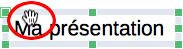
\includegraphics[angle=0,width=3cm]{./images/presentation/Impress_07DiaSansFormat_05}

\vspace{1em}

Pour modifier la taille des caractères, deux possibilités :
\begin{itemize}
\item sélectionner toute la zone de texte (\circled{1} sur la figure ci-dessous à gauche) puis choisir la taille des caractères (\circled{2}) ; 
\item sélectionner le texte uniquement (figure à droite ci-dessous), puis choisir la taille des caractères.
\end{itemize}

\deuximagesici{./images/presentation/Impress_07DiaSansFormat_03}{.9\textwidth}
	      {./images/presentation/Impress_07DiaSansFormat_04}{.9\textwidth}

Attention, parfois lorsqu'on augmente la taille des caractères (\circled{1} sur la figure ci-dessous), le cadre devient trop petit pour loger le texte sur une seule ligne (\circled{2}). Il faut alors agrandir la boîte à l'aide des poignées (figure ci-dessous à droite).

\deuximagesici{./images/presentation/Impress_07DiaSansFormat_06}{.9\textwidth}
	      {./images/presentation/Impress_07DiaSansFormat_07}{.9\textwidth}


\subsubsection{Insérer une image dans une diapositive}\index{Impress!Insérer une image}\index{Image, insérer (Impress)}\label{Presentation1image}


\begin{minipage}[c]{.68\textwidth}
Pour insérer une image, dans le menu \texttt{Insertion}, il faut choisir \texttt{Image...} (figure ci-contre). Dans la boîte de dialogue qui s'ouvre, rechercher le fichier qui contient l'image à insérer et terminer en appuyant sur le bouton \texttt{Ouvrir}.
\end{minipage}\hfill%
\begin{minipage}[c]{.28\textwidth}
\centering%
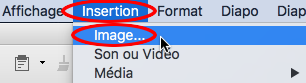
\includegraphics[angle=0,width=\textwidth]{./images/presentation/Impress_07DiaSansFormat_08}
\end{minipage}

\vspace{1em}

Lorsque l'image est sélectionnée, il est possible de modifier ses propriétés dans le panneau latéral à droite (figure ci-dessous).

\uneimageici{./images/presentation/Impress_07DiaSansFormat_09}{.8\textwidth}











\subsection{Définir une image d'arrière-plan}\index{Impress!Image d'arrière-plan}\index{Image d'arrière-plan (Impress)}\label{Presentation1imageFond}

Pour ajouter une image en arrière-plan de la diapositive, c'est-à-dire une image qui occupe tout le fond de la diapositive, deux possibilités :

\begin{itemize}
\item dans le menu \texttt{Diapo}, choisir \texttt{Définir l'image d'arrière-plan...} (figure ci-dessous à gauche) ;
\item effectuer un clic droit sur la diapositive, puis choisir dans le menu contextuel qui s'ouvre \texttt{Définir l'image d'arrière-plan} (figure ci-dessous à droite).
\end{itemize}

\deuximagesici{./images/presentation/imageAPmenu}{.8\textwidth}{./images/presentation/imageAPclicD}{.8\textwidth}

Une fois l'image choisie, une dernière boîte de dialogue s'ouvre : elle permet de choisir si l'image doit se trouver en arrière-plan d'une seule diapositive ou de toutes les diapositives.

\uneimageici{./images/presentation/imageAPboite}{.3\textwidth}



Pour supprimer une image d'arrière-plan, deux possibilités :\index{Impress!Supprimer une image d'arrière-plan}\index{Supprimer un image d'arrière-plan (Impress)}

\begin{itemize}
\item dans le menu \texttt{Diapo}, choisir \texttt{Propriétés de la page/diapo...} (figure ci-dessous à gauche) ;
\item effectuer un clic droit sur la diapositive, puis choisir dans le menu contextuel qui s'ouvre \texttt{Formater la diapo...} (figure ci-dessous à droite).
\end{itemize}

\deuximagesici{./images/presentation/imageAPsuppMenu}{\textwidth}{./images/presentation/imageAPsuppClicD}{\textwidth}

Une boîte de dialogue s'ouvre alors : choisir l'onglet \texttt{Arrière-plan} et dans la liste déroulante \texttt{Image}, sélectionner \texttt{Aucun(e)}.

\uneimageici{./images/presentation/imageAPsuppBoite}{.6\textwidth}







\subsection{Utiliser les animations}\index{Impress!Animations}\index{Animation (Impress)}\label{Presentation1effets}

Les animations permettent par exemple de faire afficher une diapositive en plusieurs temps : certaines parties de la diapositive arrivant après d'autres ou disparaissant avant le reste de la diapositive. Mais attention, il faut faire un usage parcimonieux des animations : les diaporamas en contenant trop sont souvent pénibles à suivre !

\begin{minipage}[c]{.58\textwidth}
La première étape pour ajouter une animation est de sélectionner dans la barre latérale les \texttt{Animations personnalisées} (figure ci-contre).
\end{minipage}\hfill%
\begin{minipage}[c]{.38\textwidth}
\centering%
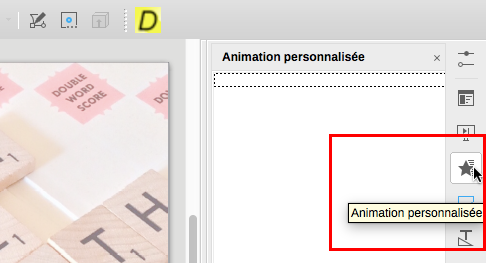
\includegraphics[angle=0,width=\textwidth]{./images/presentation/Impress_08_Transitions_01}
\end{minipage}

\vspace{1em}

\begin{minipage}[c]{.58\textwidth}
Sélectionner alors un élément de la diapositive devant être affiché après les autres, comme par exemple le texte \emph{\og À partir d'une diapositive vide \fg} (\circled{1} sur la figure ci-contre). Cliquer ensuite sur le bouton 
\includegraphics[width=.7cm]{./images/presentation/boutonPlus} (\circled{2}) pour ajouter l'effet.  
\end{minipage}\hfill%
\begin{minipage}[c]{.38\textwidth}
\centering%
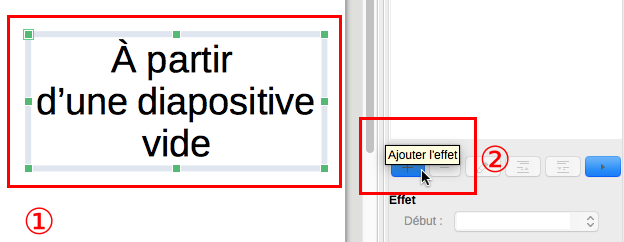
\includegraphics[angle=0,width=\textwidth]{./images/presentation/Impress_08_Transitions_02}
\end{minipage}

\vspace{1em}

\begin{minipage}[c]{.58\textwidth}
La boîte de dialogue qui s'ouvre présente le type d'animation (par exemple entrée ou sortie de l'élément sélectionné). Dans l'onglet \texttt{Entrée} (\circled{1} sur la figure ci-contre) choisir \texttt{Apparition} (\circled{2}) qui est un effet très simple permettant de faire apparaître une partie de la diapositive.
\end{minipage}\hfill%
\begin{minipage}[c]{.38\textwidth}
\centering%
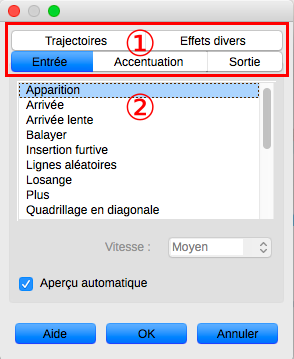
\includegraphics[angle=0,width=.7\textwidth]{./images/presentation/Impress_08_Transitions_03}
\end{minipage}


\vspace{1em}

\begin{minipage}[c]{.58\textwidth}
L'animation choisie apparaît alors dans la liste des animations (sur la figure ci-contre elle est nommé \emph{\og À partir\fg}). En la sélectionnant, il est alors possible : 
\includegraphics[width=.7cm]{./images/presentation/boutonPlus} d'ajouter une nouvelle animation sur le même élément de diapositive, 
\includegraphics[width=.7cm]{./images/presentation/boutonMoins} de supprimer l'animation, 
\includegraphics[width=.7cm]{./images/presentation/boutonCrayon} de régler les propriétés de l'animation, 
\includegraphics[width=.7cm]{./images/presentation/boutonHaut} et 
\includegraphics[width=.7cm]{./images/presentation/boutonBas} de changer l'ordre des différentes animations créées, ou encore 
\includegraphics[width=.7cm]{./images/presentation/boutonPlay} de tester l'animation choisie.    
\end{minipage}\hfill%
\begin{minipage}[c]{.38\textwidth}
\centering%
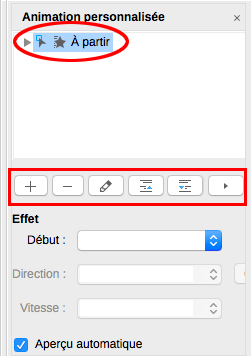
\includegraphics[angle=0,width=.7\textwidth]{./images/presentation/Impress_08_Transitions_04}
\end{minipage}

\vspace{1em}

Les animations ajoutées aux diapositives ne sont visibles que lorsque les diapositives sont affichées en mode \texttt{Diaporama}. Pour lancer le diaporama, il faut utiliser les icônes indiquées sur la figure ci-dessous. Le bouton 
\includegraphics[width=.7cm]{./images/presentation/boutonDiaporamaPlay} permet de démarrer la présentation à la première diapositive (on peut également utiliser la combinaison de touches \texttt{Fn} + \texttt{F5}. Le bouton 
\includegraphics[width=.7cm]{./images/presentation/boutonDiaporamaPause} permet de commencer le diaporama à la diapositive courante.\index{Impress!Lancer le diaporama}\index{Lancer le diaporama (Impress)}\index{Impress!Diaporama, lancer}\index{Diaporama, lancer (Impress)}

\uneimageici{./images/presentation/Impress_08_Transitions_05}{.6\textwidth}

En mode diaporama, on fait défiler les diapositives à l'aide des touches de déplacement $\leftarrow$, $\uparrow$, $\rightarrow$ et $\downarrow$ ou à l'aide des boutons de la souris. On peut aussi avec un clic droit sur le diaporama accéder directement à une diapositive précise, mettre fin au diaporama, etc. Pour sortir du mode diaporama, il faut appuyer sur la touche \texttt{Esc}.






\subsection{Ajouter des notes de présentation}\index{Impress!Notes de présentation}\index{Notes de présentation (Impress)}\label{Presentation1notes}


\begin{minipage}[c]{.68\textwidth}
Il est possible d'ajouter des \emph{\og notes \fg} associées aux diapositives. Ces notes n'apparaissent pas lors de la présentation (elles apparaissent sur l'écran secondaire s'il y en a un).

Pour ajouter des notes attachées aux diapositives il faut dans le menu \texttt{Affichage} choisir le mode \texttt{Notes} (figure ci-contre).
\end{minipage}\hfill%
\begin{minipage}[c]{.28\textwidth}
\centering%
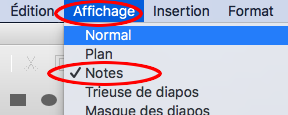
\includegraphics[angle=0,width=\textwidth]{./images/presentation/Impress_06Notes_01}
\end{minipage}

\vspace{1em}

Au pied de chaque diapositive apparaît alors une zone (figure ci-dessous à gauche) que l'on peut compléter avec le texte désiré (à droite ci-dessous).

\deuximagesici{./images/presentation/Impress_06Notes_02}{.8\textwidth}
	      {./images/presentation/Impress_06Notes_03}{.8\textwidth}








\subsection{Imprimer une présentation et ses notes}\index{Impress!Imprimer}\index{Imprimer (Impress)}\label{Presentation1export}


\begin{minipage}[c]{.58\textwidth}
Pour imprimer les diapositives et les notes associées, il faut se rendre dans le menu \texttt{Fichier} et choisir \texttt{Imprimer...} (figure ci-contre).
\end{minipage}\hfill%
\begin{minipage}[c]{.38\textwidth}
\centering%
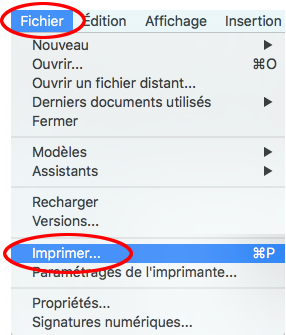
\includegraphics[angle=0,width=.7\textwidth]{./images/presentation/Impress1_impression01}
\end{minipage}

\vspace{1em}

Dans la boîte de dialogue qui s'ouvre, il est possible de choisir d'imprimer les \emph{Diapos} (figure ci-dessous), ce qui donne une impression avec une diapositive par page.

\uneimageici{./images/presentation/Impress1_impression02}{.6\textwidth}

Il est également possible de choisir le mode \emph{Prospectus}, puis de choisir le nombre de diapositives par page ainsi que leur ordre (figure ci-dessous). En face de chaque diapositive, on obtient alors des lignes permettant la prise de note.

\uneimageici{./images/presentation/Impress1_impression03}{.6\textwidth}

Il est enfin possible d'imprimer les diapositives et leurs notes en choisissant le mode \emph{Notes} (figure ci-dessous).

\uneimageici{./images/presentation/Impress1_impression04}{.6\textwidth}



\subsection{Exporter une présentation et ses notes au format PDF}\index{Impress!Exporter au format PDF}\index{Exporter au format PDF (Impress)}\label{Presentation1exportPDF}


\begin{minipage}[c]{.58\textwidth}
Pour exporter les diapositives et les notes associées au format \texttt{PDF}, il faut se rendre dans le menu \texttt{Fichier} et choisir \texttt{Exporter au format PDF...} (figure ci-contre). 
\end{minipage}\hfill%
\begin{minipage}[c]{.38\textwidth}
\centering%
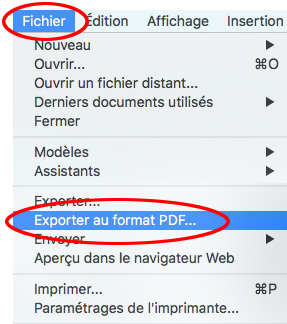
\includegraphics[angle=0,width=.7\textwidth]{./images/presentation/Impress1_exportPDF01}
\end{minipage}

\vspace{1em}

Dans la boîte de dialogue qui s'ouvre, il est possible d'exporter toutes les diapositives ou une partie seulement d'entre-elles (\circled{1} sur la figure ci-dessous). Pour exporter les notes, il faut cocher l'option \texttt{Exporter les pages de notes} \circled{2}.

\uneimageici{./images/presentation/Impress1_exportPDF02}{.7\textwidth}


Lorsque l'on exporte les notes, le document obtenu contient d'abord les diapositives (une par page), puis les notes associées (figure ci-dessous).

\uneimageici{./images/presentation/Impress1_exportPDF03}{.7\textwidth}










%
%
% SEANCE  1
%
%

\pagebreak

\section{Séance 1 : une présentation}\label{fichePresentation6e1}



\boiteEnonceLarge{Le but de cette séance est créer une présentation à l'aide du logiciel \emph{LibreOffice Impress}.



Une fois votre travail terminé, rendre le fichier au format ODP sur la plateforme \emph{Moodle} à l'endroit indiqué par votre enseignant (si nécessaire, se reporter à la fiche méthode \emph{Remettre un devoir sur Moodle}, section \vref{MoodleRendreDevoir}).


}% fin énoncé

\vfill

\cadre{Pensez à sauver régulièrement votre travail en appuyant sur \texttt{Cmd + S} ou à partir du menu \texttt{Fichier} en choisissant \texttt{Enregistrer}.

\uneimageici{./images/generales/clavierCmdS}{.3\textwidth}
}




